\subsection{Specific Aim 2: Hydrodynamics}
\label{subsec:specific_aim_2}
In Specific Aim 2, we include hydrodynamics effects by embedding the particles in a solvent. 
As described in \eqref{eq:stokes} and illustrated in Figure \ref{fig:flow_map}, 
the solvent phase is modeled by the Stokes equations for an incompressible, zero Reynolds-number fluid, 
and these equations are coupled to the screened-Laplace equation \eqref{SL} through viscous and hydrophobic stress balance.
Hydrodynamic effects are a relevant detail  
because the rates of biological functions like fusion, fission, and pore dynamics rely on viscous dissipation \cite{RYHAM20112929}. 
%While hydrophobic attraction causes the particles to self-assemble indepedently of the dissipation mechanism, the trajectories and
%equilibrium configurations depend on the fact that the particles travel through a viscous environment. 
Additionally, hydrodynamics interactions are central fabrication of complex microscopic three-dimensional structures \cite{Cho2010}.
Over the past decade, there has been an explosion of interest in small-scale processes that utilize capillary forces dominate,  van der Waals interactions and thermal noise  \cite{Zhang2017}, to coordinated movement and bind  material subunits, \cite{Pandey2011,Leong2007,Reynolds2019, Dasgupta2017,Siontorou2017}.
Finally, coarse-grained and molecular dynamics theories include water either explicitly or implicitly in their models. 
The immediate goal of the present proposal
is to be able to simulate vesicle bilayers in external flows, where the bilayers are represented by a self-assembled collection of rigid particles.

\begin{figure}[h]
  \centering{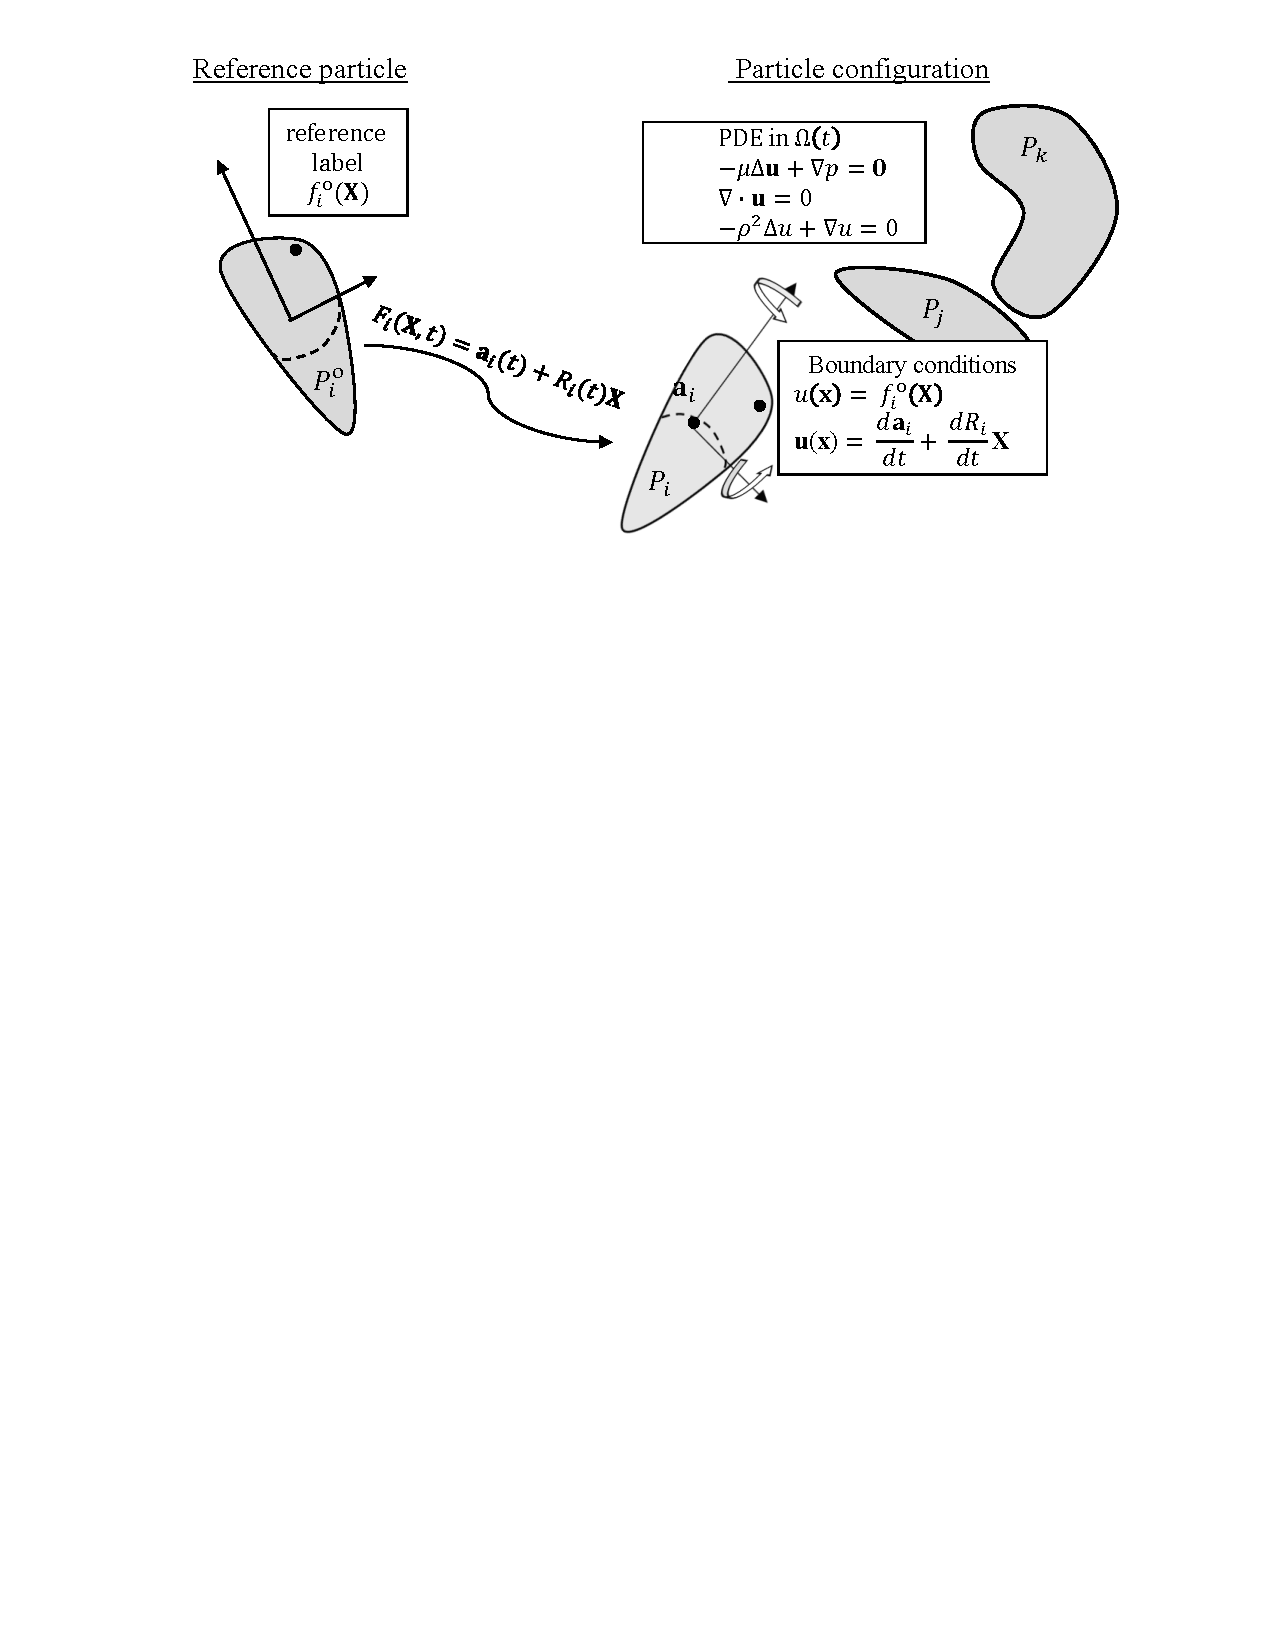
\includegraphics[width=0.8\textwidth]{Figures/domain.pdf}}
    \caption{\label{fig:flow_map}}
\end{figure}


%We must solve the system 
%\setcounter{midequation}{\theequation}
%\addtocounter{midequation}{2}
%\begin{minipage}[t]{0.44\textwidth}
%\begin{subequations}
%\begin{alignat}{2}
%\label{St1} -& \mu \Delta {\bf u} + \nabla p = {\bf 0}, \\
%\label{St2}  & \nabla \cdot {\bf u} = 0,                &&   \text{in } \Omega\\
%\label{St3}  & {\bf u }({\bf x}) = {\bf v}_i + {\bf w_i}\times {\bf x}, \;  && \text{for } {\bf x} \in \partial P_i\\
%\label{St4}  & ({\bf u } - {\bf u}_{\infty})({\bf x}) \to {\bf 0} && \text{as } {\bf x} \to \infty\\
%\notag \\
%\tag{\themidequation}
%\label{HSB1}  & \int_{\partial P_i} \boldsymbol{\sigma} \boldsymbol{\nu} \,\dif S + {\bf F}_{i} = {\bf 0}\span \span
%\end{alignat}
%\end{subequations}
%\end{minipage}
%\addtocounter{equation}{1}
%\setcounter{midequation}{\theequation}
%\addtocounter{midequation}{2}
%\begin{subequations}
%\begin{minipage}[t]{0.5\textwidth}
%\begin{alignat}{2}
%\label{SL1}  - & \rho^2 \Delta u +u = 0, && \text{in } \Omega\\
%\label{SL2}   & u({\bf x}) = f_i({\bf x}),\quad  && \text{for } {\bf x} \in \partial P_i\\
%\label{SL3} &  u({\bf x}) \to 0 && \text{as } {\bf x} \to \infty \\
%\notag \\
%\notag \\
%\tag{\themidequation}
%\label{HSB2}   & \int_{\partial P_i} {\bf x} \times \boldsymbol{\sigma} \boldsymbol{\nu} \,\dif S + {\bf G}_{i} = {\bf 0} \span \span\\
%\notag
%\end{alignat}
%\end{minipage} 
%\end{subequations}
%\noindent for $i = 1,\dots, N$.

\textbf{Vesicles in background flows.}
Numerically solving the Stokes-screened Laplace system \eqref{SL}, \eqref{eq:stokes} is a nontrivial matter,
and we will develop an efficient, robust, high-order of accuracy in time and space algorithm suited to the problem. 
The challenges are: \textbf{(1)} the equations express a two-way coupling.
This means that the flow changes the shape of the bilayer (or particle suspension, more generally),
and in return the hydrophobic stresses coming from the altered shape imparts a force on the flow. 
\textbf{(2)}
The inputs to the Stokes equations are particle configurations, forces and torques. 
The outputs are the rigid body translation and angular velocties used to update the particle positions (see Figure \ref{fig:flow_map}).
Although the underlying equations are linear, the overall problem is highly nonlinear because the domain is constantly changing.
\textbf{(3)} Self-assembly causes the particles to come into close contact.  
As a result, a exceptional spatial accuracy is required to resolve the fields between adjacent particles.
Finally, the physically relevant elastic properties of bilayer become apparent at large length scales and for large particle-numbers,
which increases the computational complexity of our simulations. 

We include a background flow by replacing the third equation in \eqref{eq:stokes} with the condition
$(\mathbf{u} - \mathbf{u}_{\infty})(\mathbf{x}) \to \mathbf{0}$ as $|\mathbf{x}| \to \infty.$ 
One way to ensure this far-field condition is through the represention 
\begin{equation}
\label{PowerMiranda}
{\bf u} = {\bf u}_{\infty} + D\eta + \sum_{i=1}^N S(\cdot, {\bf a}_i) {\bf F}_i + R(\cdot, {\bf a}_i) {\bf G}_i.
\end{equation}
where $S$ and $R$ are stokeslets and rotlets supported at the respective particle centers 
and $D\eta$ is an appropriate double layer integral operator for an unknown density function $\eta.$ 
The representation \eqref{PowerMiranda} automatically satisfies all equations with the exception of the rigid motion boundary conditions. 
These conditions follow by requiring the viscous stress vanishes across the particle boundaries.

We will compare the behavior of our particle-based vesicles in Stokes flow to well-established results.
\todo{What are the known results?}
To test area incompressibility, we form the bilayer midplane by fitting to the particle centers. Under moderate shear rates,
the vesicle elongates and takes on an elliptical shape. We will study the increase in midplane area as a function of shear rate.
Additionally, we will test for tangential divergence of velocity.
Researchers have devised to model area incompressible and
volume conserving membranes
\cite{torres-sanchez_millan_arroyo_2019, mahapatra_saintillan_rangamani_2020, Steigmann99, C6SM02452A}.
Our preliminary results show that the particle-based bilayers have the same area modulus, about 60 \kBT,  as that of real lipid bilayer membranes,
and so we expect realistic results from our flow simulations with regard to area incompressibility.  It is noteworthy that
area incompressibility is some sense baked into the model through the hydrophobic attraction. 

Bilayer membranes have a small permeability to water \cite{323e9a2f0c58487ea82518d7a1f96485},
and so modelers often assume a vesicle membrane that conserves volume. In our particle-based approach, water motion across
the bilayer is limited by the size of the gaps between the particles, which is an artifact of coarse-graining.
Making these gaps smaller comes at the expense of numerical accuracy, and so we will assess if there is a reasonable trade-off
between approximate volume conservation and simulation complexity. 

\begin{wrapfigure}[16]{r}{0.32\textwidth}
\centerline{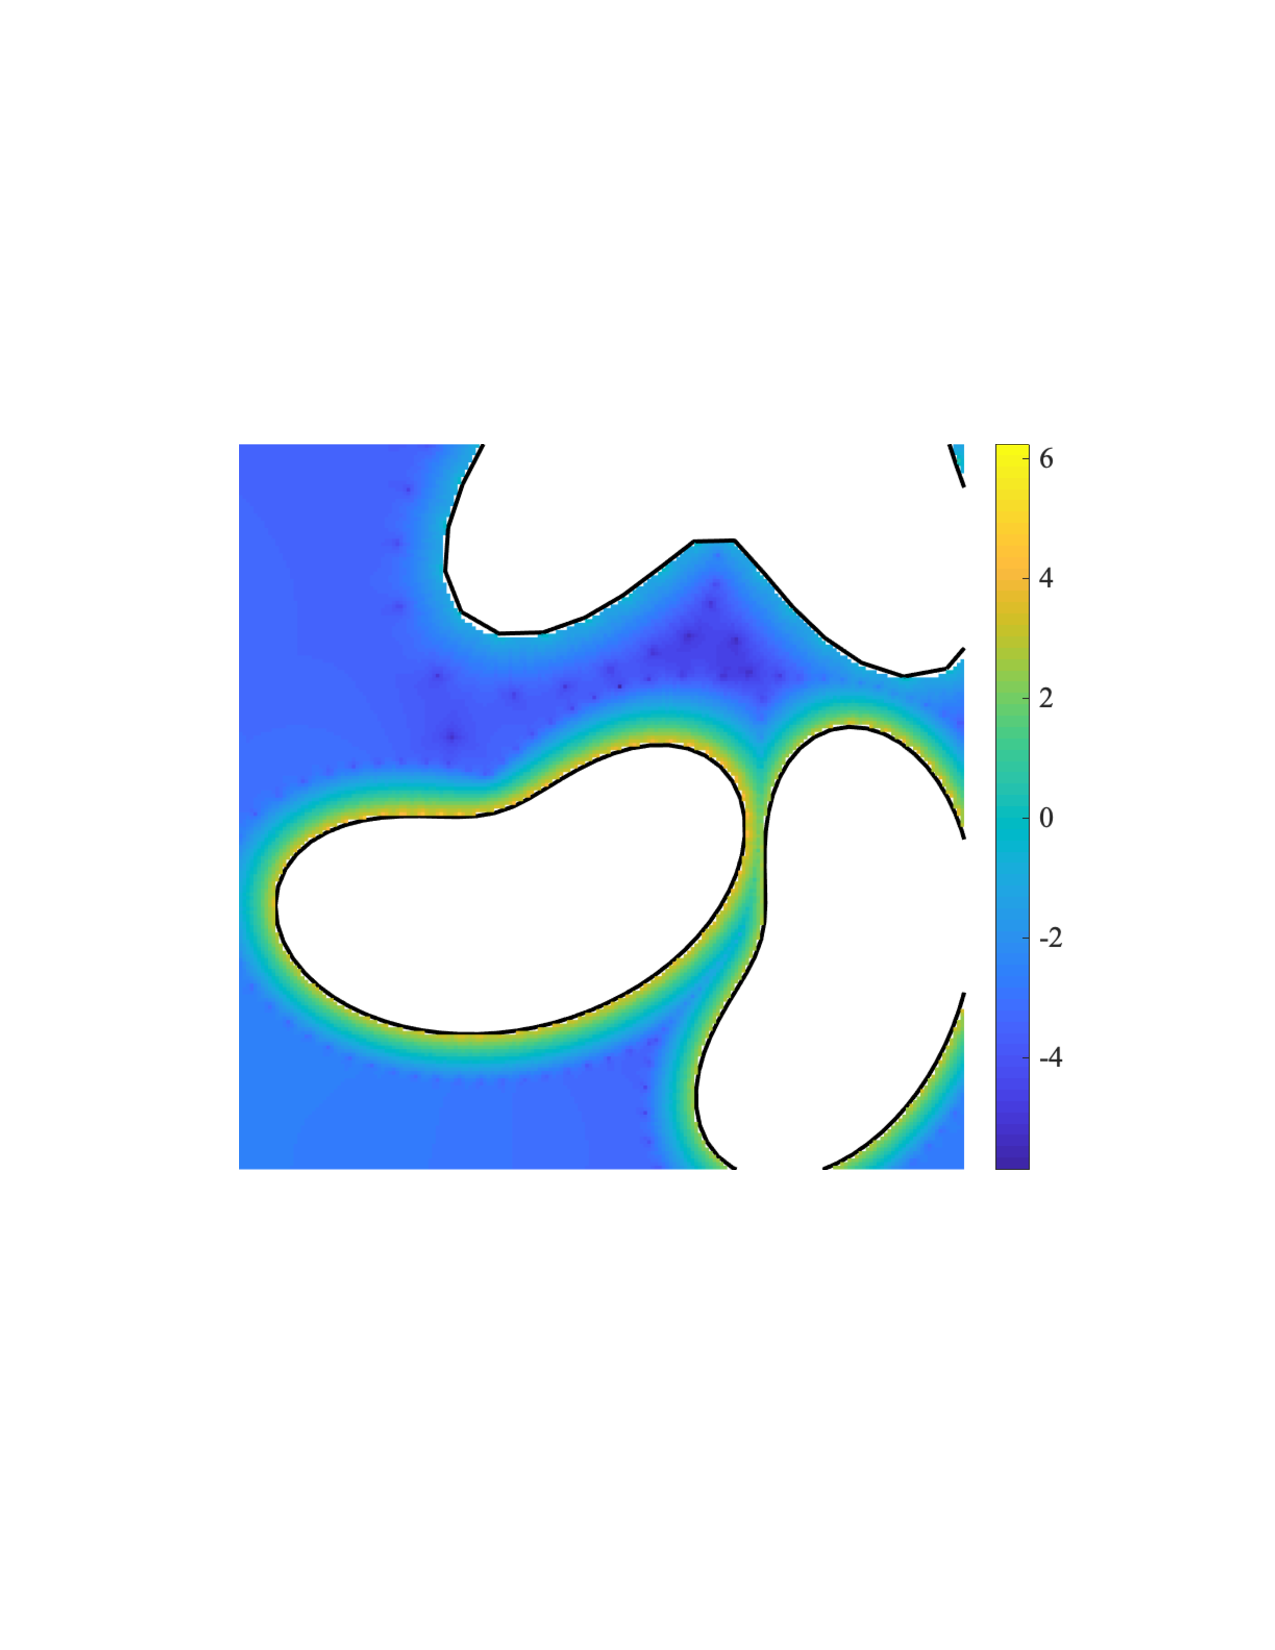
\includegraphics[width=0.32\textwidth]{figures/BIError.pdf}}
\caption{
\label{fig:bierror}  
  Gradient error between an exact and boundary integral solution of \eqref{SL}.
}
\end{wrapfigure}

Finally, the particle-based vesicle bilayers have two distinct leaflets.
The inner and outer leaflets consists of the particles in contact with the vesicle interior and 
surrounding fluid respectively. Since there the separation between these layers is roughly fixed,
about 2 nm, certain fluid mechanical effects arise that are not present in zero-thickness membrane models. 
An important effects we observe is that the leaflets slide against one another under shear flow. 
This implies that part of the viscous dissipation in the aqueous phase is enhanced by intermonolayer friction
\cite{SHKULIPA2005823, ShkulipaThesis}. We will characterize the intermonolayer
slip as a function of shear rate, vesicle diameter and particle geometry. 

\textbf{Novel reciprocal relations.}
We use a double layer The velocity field  double layer potential representation.
This representation involves a strongly singular integral, and without the aid of specilized
quadrature routines, leads to large numerical errors when evaluating the the hydrophobic stress \eqref{stress} along the particle boundaries (see Figure \cite{fig:bierror}).
We prove a, to our knowledge new, result concerning the evaluation of Maxwell-type stresses. 
\begin{proposition}
  \label{prop:recip}
  Suppose that $u = \sum_{i=1}^N u_i$ where $u_i$ is a solution of the screened Laplace equation
  in $\mathbb{R}^3 \setminus P_i$ for $i=1,\dots, N.$ Then 
  \begin{equation}
    \label{eq:reciprocal}
{\bf F}_i = \sum_{j \neq i} \int_{\partial P_i}[\boldsymbol{\sigma}_{ij} + \boldsymbol{\sigma}_{ji}]\boldsymbol{\nu}\,\dif S,\quad
{\bf G}_i = \sum_{j \neq i} \int_{\partial P_i} {\bf x} \times [\boldsymbol{\sigma}_{ij} + \boldsymbol{\sigma}_{ji}]\boldsymbol{\nu}\,\dif S, \quad i = 1\dots, N.
\end{equation}
where $\boldsymbol{\sigma}_{ij} = \rho^{-1} u_iu_j {\bf I} + \rho(\nabla u_i \cdot \nabla u_j {\bf I} - 2 \nabla u_i \otimes \nabla u_j)$ and
$[\cdot]$ denotes the jump in stress across $\partial \Omega.$ 
\end{proposition}


The identity in Proposition \ref{prop:recip} gets around this critical issue by utilizing the fact that $u_j$, $j\neq i$ is smooth and the normal derivative
of  $u_i$ continuous across $\partial P_i$. Despite the large gradient errors in Figure \ref{fig:bierror}, the force and torque
calculated by \eqref{eq:reciprocal} achieved $10^{-4}$ accuracy.



